\subsection{Configuração com Um Servidor \textit{Web}}

\paragraphnl{Resultados obtidos}

São apresentados em seguida sob a forma de uma tabela e de um gráfico os dados recolhidos para a configuração do serviço com \textbf{um} servidor web, nomeadamente o número de pedidos por segundos (débito) e a percentagem de pedidos falhados. \\

\begin{table}[!h]
\centering
\begin{tabular}{|c|c|c|}
\hline
\textbf{\# Clientes} & \textbf{Pedidos/s} & \textbf{\% Pedidos Falhados} \\ \hline
1 & 21.30 & 0 \\ \hline
2 & 25.42 & 0 \\ \hline
4 & 25.62 & 0 \\ \hline
8 & 26.41 & 0 \\ \hline
16 & 26.64 & 0 \\ \hline
32 & 24.03 & 0 \\ \hline
64 & 17.76 & 0 \\ \hline
128 & 12.28 & 23 \\ \hline
\end{tabular}
\caption{Tabela com débito e percentagem de pedidos falhados em função do número de clientes (1 Web Server)}
\end{table}

\begin{figure}[!h]
\centering
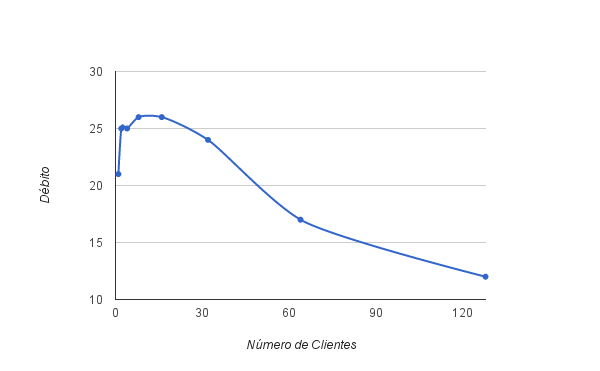
\includegraphics[scale=.6]{img/ab/web1.png}
\caption{Débito obtido de acordo com o número de clientes (1 Web Server)}
\end{figure}

\newpage
\paragraphnl{Análise aos resultados obtidos}

O débito obtido para esta onfiguração em concreto aumenta, ainda que muito timidamente, até 16 clientes em simultâneo.
A diferença de um para cliente para 16 clientes em simultâneo é pouco significativa. \\

A partir de 32 \textit{threads} em simultâneo, assiste-se a uma degradação da \textit{performance}.
Esta queda no débito culmina com um valor fraco de $12.28$ pedidos/segundo, para 128 clientes.
A acrescentar a este facto, verifica-se também que cerca de um quarto dos pedidos efetuados pela ferramenta de \textit{benchmark} ao único servidor \textit{web} não foram, sequer, atendidos por este. \\

Assim, pode-se afirmar, para esta configuração, que o serviço não responde eficazmente ao progressivo aumento do número de utilizadores.
Este facto acaba por ser visto como uma situação perfeitamente normal e esperada, dado que apenas um servidor foi destacado para operacionalizar o serviço.

%% 2 SERVIDORES WEB

\subsection{Configuração com Dois Servidores \textit{Web}}

\paragraphnl{Resultados obtidos}

São apresentados em seguida sob a forma de uma tabela e de um gráfico os dados recolhidos para a configuração do serviço com \textbf{dois} servidores web, nomeadamente o número de pedidos por segundos (débito) e a percentagem de pedidos falhados. \\

\begin{table}[!h]
\centering
\begin{tabular}{|c|c|c|}
\hline
\textbf{\# Clientes} & \textbf{Pedidos/s} & \textbf{\% Pedidos Falhados} \\ \hline
1 & 24.45 & 0 \\ \hline
2 & 47.54 & 0 \\ \hline
4 & 51.02 & 0 \\ \hline
8 & 48.16 & 0 \\ \hline
16 & 49.47 & 0 \\ \hline
32 & 25.32 & 0 \\ \hline
64 & 19.20 & 0 \\ \hline
128 & 28.74 & 30 \\ \hline
256 & 39.17 & 34 \\ \hline
\end{tabular}
\caption{Tabela com débito e percentagem de pedidos falhados em função do número de clientes (2 Web Servers)}
\end{table}

\newpage

\begin{figure}[!h]
\centering
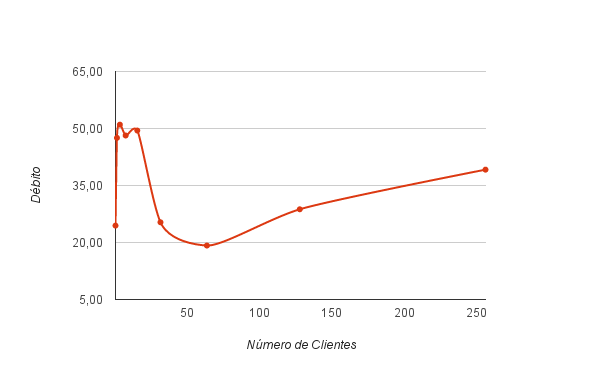
\includegraphics[scale=.6]{img/ab/web2.png}
\caption{Débito obtido de acordo com o número de clientes (2 Web Servers)}
\end{figure}

\paragraphnl{Análise aos resultados obtidos}

Verifica-se que, para uma configuação com dois servidores \textit{web}, o valor do débito máximo atingido ocorre para 16 clientes em simultâneo.
Este valor dobra o atingido para um único cliente e, também, é quase o dobro do máximo registado para a configuração com um único \textit{web server}. \\

No entanto, a partir dos 16 clientes, e até aos 64, regista-se um decréscimo deste.
Ora, o débito voltar a subir para 128 e 256, acompanhados, é verdade, de uma alta percentagem de pacotes falhados.
Este facto apresenta-se como um problema com relevo no serviço, mas também justificável pela sobrecarga causada por um número mais elevado de clientes. \\

Pode-se observar, deste modo, que para 256 clientes em simultâneo, o débito obtido é positivo e vai de encontro às expectativas, já que quase dobrou o valor máximo atingido na configuração analisada anteriormente.
Verifica-se também, com alguma estranheza, a queda do débito obtido para 64 \textit{hosts}.
Este valor pode ser justificado como um \textit{outlier}, levando a que, de forma ideal, o teste em particular devesse ser repetido.
No entanto, e dada as restições de tempo na elaboração do trabalho, não foi possível verificar esta assunção.

\newpage
\subsection{Configuração com Três Servidores \textit{Web}}

\paragraphnl{Resultados obtidos}

São apresentados em seguida sob a forma de uma tabela e de um gráfico os dados recolhidos para a configuração do serviço com \textbf{três} servidores web, nomeadamente o número de pedidos por segundos (débito) e a percentagem de pedidos falhados. \\

\begin{table}[!h]
\centering
\begin{tabular}{|c|c|c|}
\hline
\textbf{\# Clientes} & \textbf{Pedidos/s} & \textbf{\% Pedidos Falhados} \\ \hline
1 & 25.18 & 0 \\ \hline
2 & 49.00 & 0 \\ \hline
4 & 43.94 & 0 \\ \hline
8 & 64.05 & 0 \\ \hline
16 & 62.30 & 0 \\ \hline
32 & 29.43 & 0 \\ \hline
64 & 43.57 & 0 \\ \hline
128 & 31.41 & 0 \\ \hline
256 & 28.51 & 0 \\ \hline
512 & 43.40 & 47 \\ \hline
\end{tabular}
\caption{Tabela com débito e percentagem de pedidos falhados em função do número de clientes (3 Web Servers)}
\end{table}

\begin{figure}[!h]
\centering
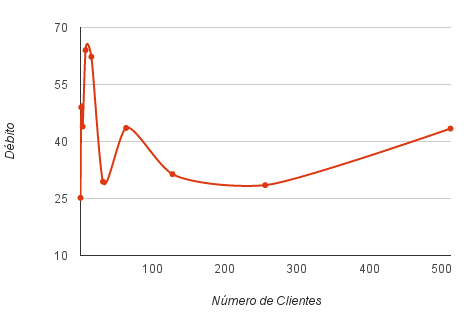
\includegraphics[scale=.6]{img/ab/web3.png}
\caption{Débito obtido de acordo com o número de clientes (3 Web Servers)}
\end{figure}

\newpage

\paragraphnl{Análise aos resultados obtidos}

O primeiro facto a registar é a obtenção de um novo valor máximo para o débito, quando comparado com configurações previamente analisadas.
Este valor situa-se na casa dos $65 pedidos/segundo$ e ocorre para $8$ clientes ligados de forma concorrente.
A ocorrência de tal valor demonstra que o \textit{cluster} ainda apresenta capacidade para escalar na oferta do seu serviço \textit{web}.
Até aqui, esta tem sida uma tendência dominante. \\

No entanto, há que destacar, por um lado, a queda abrupta deste valor para um número maior de clientes ($128$) e a impactante percentagem de pacotes perdidos com $512$ clientes connectados em simultâneo.
Este é um número demasiado relevante para ser ignorado, o que leva a crer que a atual configuração ainda não estará pronta para dar resposta a uma quantidade substancialmente grande de utilizadores ligados concorrentemente.

\subsection{Configuração com Quatro Servidores \textit{Web}}

\paragraphnl{Resultados obtidos}

São apresentados em seguida sob a forma de uma tabela e de um gráfico os dados recolhidos para a configuração do serviço com \textbf{quatro} servidores web, nomeadamente o número de pedidos por segundos (débito) e a percentagem de pedidos falhados. \\

\begin{table}[!h]
\centering
\begin{tabular}{|c|c|c|}
\hline
\textbf{\# Clientes} & \textbf{Pedidos/s} & \textbf{\% Pedidos Falhados} \\ \hline
1 & 25.79 & 0 \\ \hline
2 & 46.58 & 0 \\ \hline
4 & 68.22 & 0 \\ \hline
8 & 64.25 & 0 \\ \hline
16 & 66.57 & 0 \\ \hline
32 & 69.28 & 0 \\ \hline
64 & 46.27 & 0 \\ \hline
128 & 58.63 & 0 \\ \hline
256 & 34.06 & 0 \\ \hline
512 & 44.95 & 8 \\ \hline
\end{tabular}
\caption{Tabela com débito e percentagem de pedidos falhados em função do número de clientes (4 Web Servers)}
\end{table}

\newpage

\begin{figure}[!h]
\centering
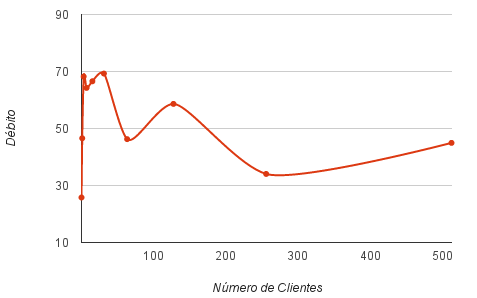
\includegraphics[scale=.6]{img/ab/web4.png}
\caption{Débito obtido de acordo com o número de clientes (4 Web Servers)}
\end{figure}

\paragraphnl{Análise aos resultados obtidos}

Os dados exibidos na tabela e suportados pelo desenho do gráfico, de facto, não enganam.
Estes são os melhores resultados globais, a todos níveis, obtidos até ao momento.
Não se tinha conseguido, até então, estar tão consistentemente na gama de valores para o débito entre os $60$ e $70$ pedidos/segundo. \\

Observa-se, para além disto, que também foi atingido um novo valor máximo para esta métrica.
O valor é de, aproximadamente, $70$ pedidos/segundo e ocorre para $32$ clientes, quando na configuração anterior, com três servidores \textit{web}, este valor verificou-se para $8$ clientes em simultâneo. \\

Comparando o rendimento para $512$ clientes com a configuração anterior, verifica-se que o débito de ambos é extremamente semelhante, mas a taxa de perda de pacotes é drasticamente supeior na configuração analisada anteriormente.
Esta é, sem sombra de dúvida, uma excelente melhoria para o serviço prestado pela infrestrutura.


\newpage
\subsection{Configuração com Seis Servidores \textit{Web}}

São apresentados em seguida sob a forma de uma tabela e de um gráfico os dados recolhidos para a configuração do serviço com \textbf{seis} servidores web, nomeadamente o número de pedidos por segundos (débito) e a percentagem de pedidos falhados. \\

\paragraphnl{Resultados obtidos}

\begin{table}[!h]
\centering
\begin{tabular}{|c|c|c|}
\hline
\textbf{\# Clientes} & \textbf{Pedidos/s} & \textbf{\% Pedidos Falhados} \\ \hline
1 & 19.06 & 0 \\ \hline
2 & 34.40 & 0 \\ \hline
4 & 15.95 & 0 \\ \hline
8 & 50.40 & 0 \\ \hline
16 & 57.85 & 0 \\ \hline
32 & 57.04 & 0 \\ \hline
64 & 26.83 & 0 \\ \hline
128 & 18.01 & 0 \\ \hline
256 & 33.70 & 0 \\ \hline
512 & 45.13 & 7 \\ \hline
\end{tabular}
\caption{Tabela com débito e percentagem de pedidos falhados em função do número de clientes (6 Web Servers)}
\end{table}

\begin{figure}[!h]
\centering
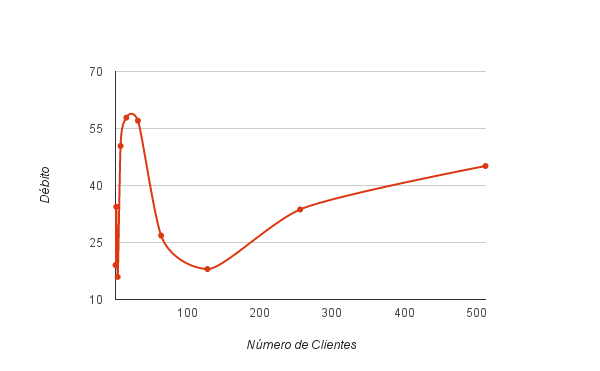
\includegraphics[scale=.6]{img/ab/web6.png}
\caption{Débito obtido de acordo com o número de clientes (6 Web Servers)}
\end{figure}

\newpage
\paragraphnl{Análise aos resultados obtidos}

Os dados obtidos mostram, inequivocamente, que a \textit{performance} do servidor piorou com uma configuração de seis servidores \textit{web} em relação à configuração com apenas quatro. \\

O valor máximo de débito atingido não excedeu os $60$ pedidos/segundo, o que é inferior ao registado na configuração anterior.
Os valores médios desta métrica em função do número de clientes em simultâneo apresentam também piores resultados do que os observados na configuração anterior. \\

Deste modo, é correto afirmar que a configuração anterior será a configuração ideal será a com quatro servidores \textit{web}.
Este facto será evidenciado já na secção seguinte, onde será realizada uma comparação entre todas as configurações abordadas neste projeto. \\

Uma justificação plausível para esta quebra de rendimento da infraestrutura para esta configuração pode dever-se à falta de recursos computacionais da máquina fisíca em que estavam em execução as máquinas virtuais respeitantes a este servidores.

\newpage
\subsection{Comparação das Configurações Analisadas}

É abaixo exibido o gráfico global e comparativo dos valores do débito obtidos para todas as configurações relativas ao número de servidores \textit{web} que a infraestrutura deverá apresentar. \\

\begin{figure}[!h]
\centering
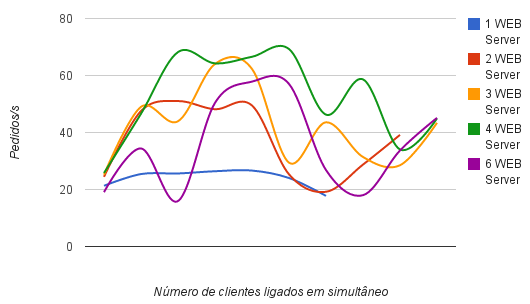
\includegraphics[scale=.6]{img/ab/web-compare.png}
\caption{Comparação do débito obtido em função do número de clientes para as várias configurações}
\end{figure}

Como já se fazia adivinhar, e como já fora comentado na parte final da secção anterior, a configuração que melhor resultados apresenta é a com \textbf{quatro} servidores \textit{web}. \\

Este facto pode ser justificado por uma análise aos recursos fisícos da máquina onde todos os servidores \textit{web} foram executados.
O processador desta é composto por quatro núcleos (\textit{quad-core}), e estando designada a cada máquina virtual um \textit{core}, é natural que a performance da infraestrutura atinga o seu pico quando apenas os quatro servidores estiverem em execução.
Um número maior do que quatro servidores implica partilha dos recursos computacionais, resultando num \textit{overhead} computacional gasto na gestão de execução de processos pelo sistema operativo da máquina fisíca (\textit{context-switching}). \\

O valor de débito máximo obtido foi de $69.28 pedidos/segundo$ e ocorreu para 32 clientes em simultâneo, na configuração com quatro servidores \textit{web}.
